\documentclass[12pt, a4paper]{article}
\usepackage[utf8]{inputenc} 
\usepackage{authblk}
\usepackage{multicol}
\usepackage{multirow}
\usepackage{url}
\usepackage{graphicx}
\usepackage{amsfonts}
\usepackage[tbtags]{amsmath}
\usepackage{caption}
\usepackage{subcaption}
\title{CSE 300: Online Assignment}
\author{Md Shamsuzzoha Bayzid, Mahjabin Nahar, Md Shariful Islam Bhuyan,
	and Md Saidur Rahman}
\date{June 2021}


\begin{document}
	\maketitle
	\section{Introduction}
	This assignment has been designed to assess the preparation of the students
	in writing scientific articles using \LaTeX. This assignment covers a variety of
	components that are commonly used in scientific manuscripts.
	\subsection{Equations}
	Let $C$ be a simple piecewise smooth curve that bounds a region $D$ in the
	plane. If $P\left(x,y\right)$ and $Q\left(x,y\right)$ have continuous partials in an open region
	containing $D$, then\\
	$ \int_{C}Pdx + Qdy = \iint_{D} \frac{\partial Q}{\partial x} -\frac{\partial P}{\partial y} dA  $
	\par
	If $\mathrm{\textbf{F}}$ is a vector field with third component 0 defined on a domain $D$
	enclosed by boundary $C$ then\\
	$ \oint_{C} \mathrm{\textbf{F}}\cdot d\mathrm{\textbf{r}} = \iint_{D} \left(\nabla \times \mathrm{\textbf{F}} \right) \cdot \mathrm{\textbf{k}}dA. $
	\par
	Similarly, if $C$ is defined by $\mathrm{\textbf{r}}(t) = \langle
	x(t), y(t)\rangle	$\\
	$ \oint_{C} \mathrm{\textbf{F}}\cdot \mathrm{\textbf{n}} ds = \iint_{D} \nabla \cdot \mathrm{\textbf{F}} dA $
	
	\subsection{Tables}
	We wish to place the Table at the bottom of the page.
	\subsection{Figures}
	We intend to put Figure \ref{fg:fg1} at the top of a page.
	
	\section{Conclusions}
	The major objectives of this assignment are listed below (please do not ignore
	the font sizes).
	\begin{itemize}
		\item {\Large To assess the ability of the students in preparing
			manuscripts in \LaTeX.}
		 {\Large \item} {\large To see if the students have adequately practiced different
			aspects of writing in \LaTeX.}
		{\large \item} To see if the students can add various basic components (e.g., tables,
		figures, equations) to a {\LaTeX} manuscript.
		\item {\small To see if the students can leverage the available materials (both offline and
			online) to do something which has not explicitly been taught in the class.}
	\end{itemize}
	
	\begin{table}[b]
		\begin{tabular}{|l||l|l|l|}
			\hline
			\multicolumn{4}{|c|}{Item List}\\
			\hline
			Item~~~ Name~~~ or  &\multirow{2}{*}{ALPHA 2 Code~~~} &\multirow{2}{*}{ALPHA 3 Code~~~} &\multirow{2}{*}{Numeric Code~~~} \\
			Product Name & & & \\
			\hline
			\multirow{2}{*}{Item001} & \multirow{2}{*}{AF} & \multirow{2}{*}{AFG} & 001\\
			& & & 002 \\
			\hline
			Item002& AX &ALA &003\\
			\hline
			\multirow{2}{*}{Item003} & \multirow{2}{*}{AL} & \multirow{2}{*}{ALB} & 004\\
			& & & 005 \\
			& & & 006 \\
			& & & 008 \\
			\hline
			\multirow{2}{*}{Item004} & \multirow{2}{*}{DZ} & \multirow{2}{*}{DZA} & 009\\
			& & & 010 \\
			\hline
			\multirow{2}{*}{Item005} & \multirow{2}{*}{AS} & \multirow{2}{*}{ASM} & 011\\
			& & & 012 \\
			\hline
			Item006 & AD & AND & 013\\
			\hline
			Item007& AO& AGO& 014\\
			\hline
			\hline
		\end{tabular}
	\end{table}
	
	\begin{figure}[t]
		\centering
		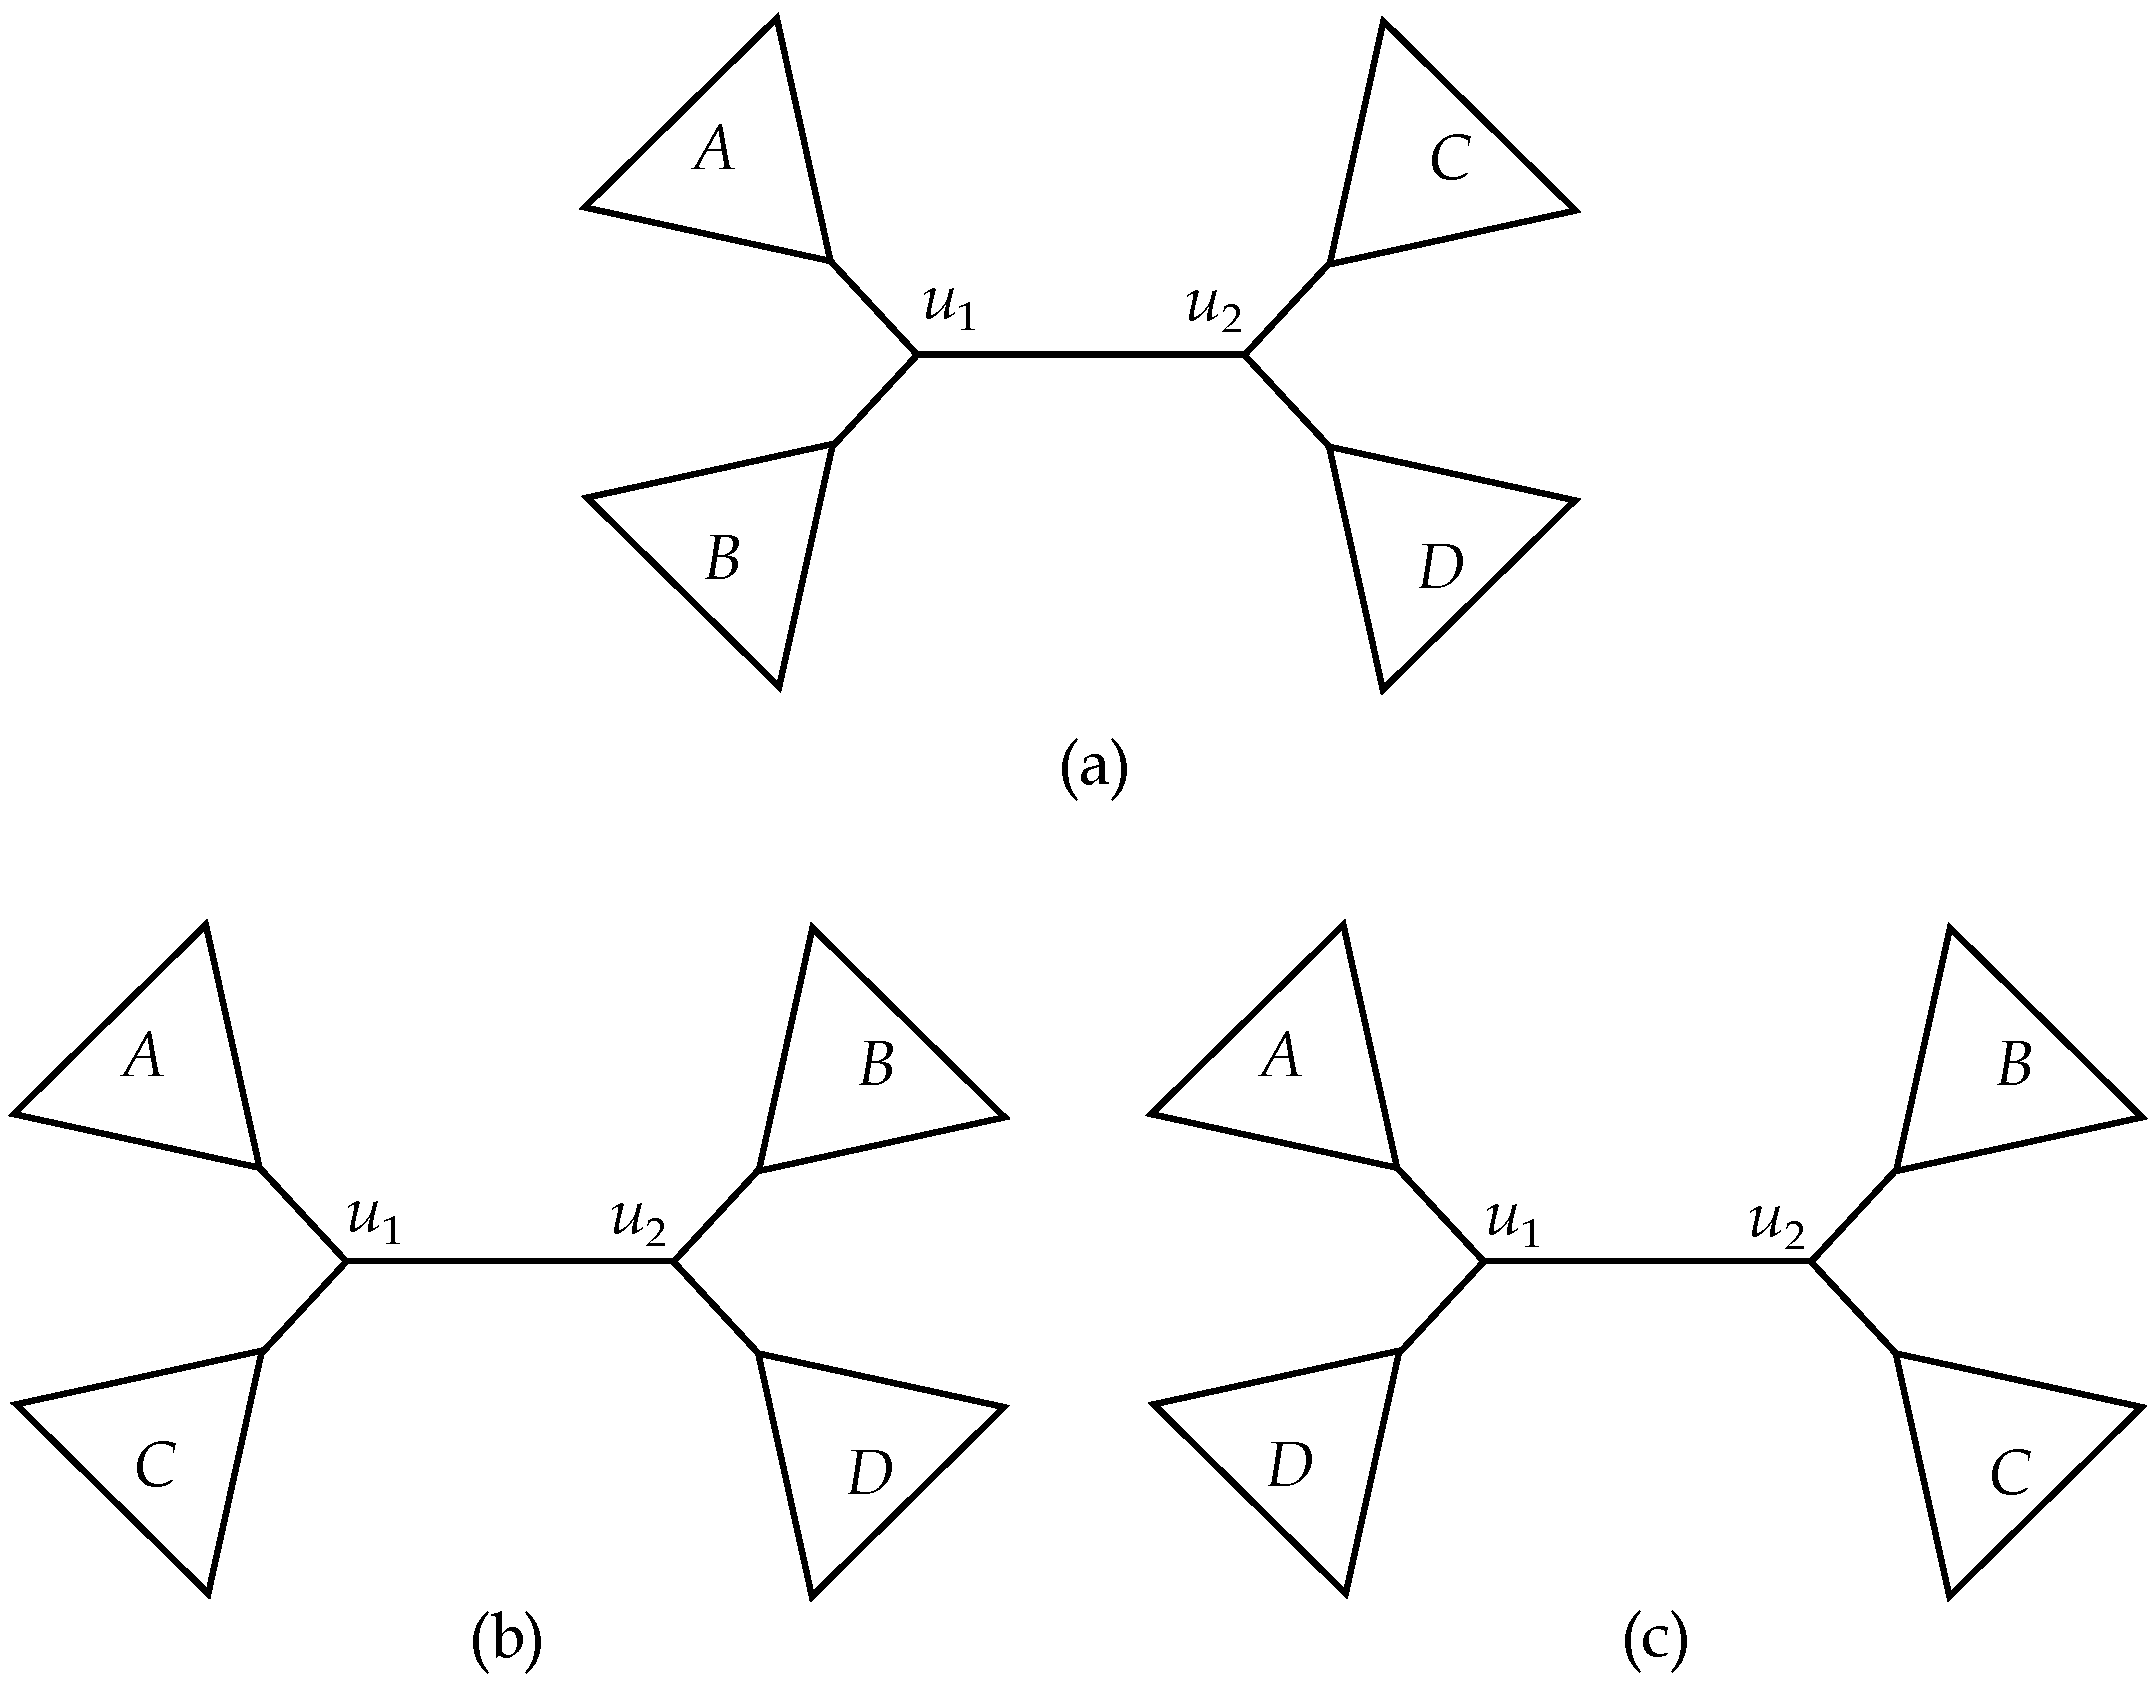
\includegraphics[scale=0.33, angle =180 ]{Figure3.pdf}
		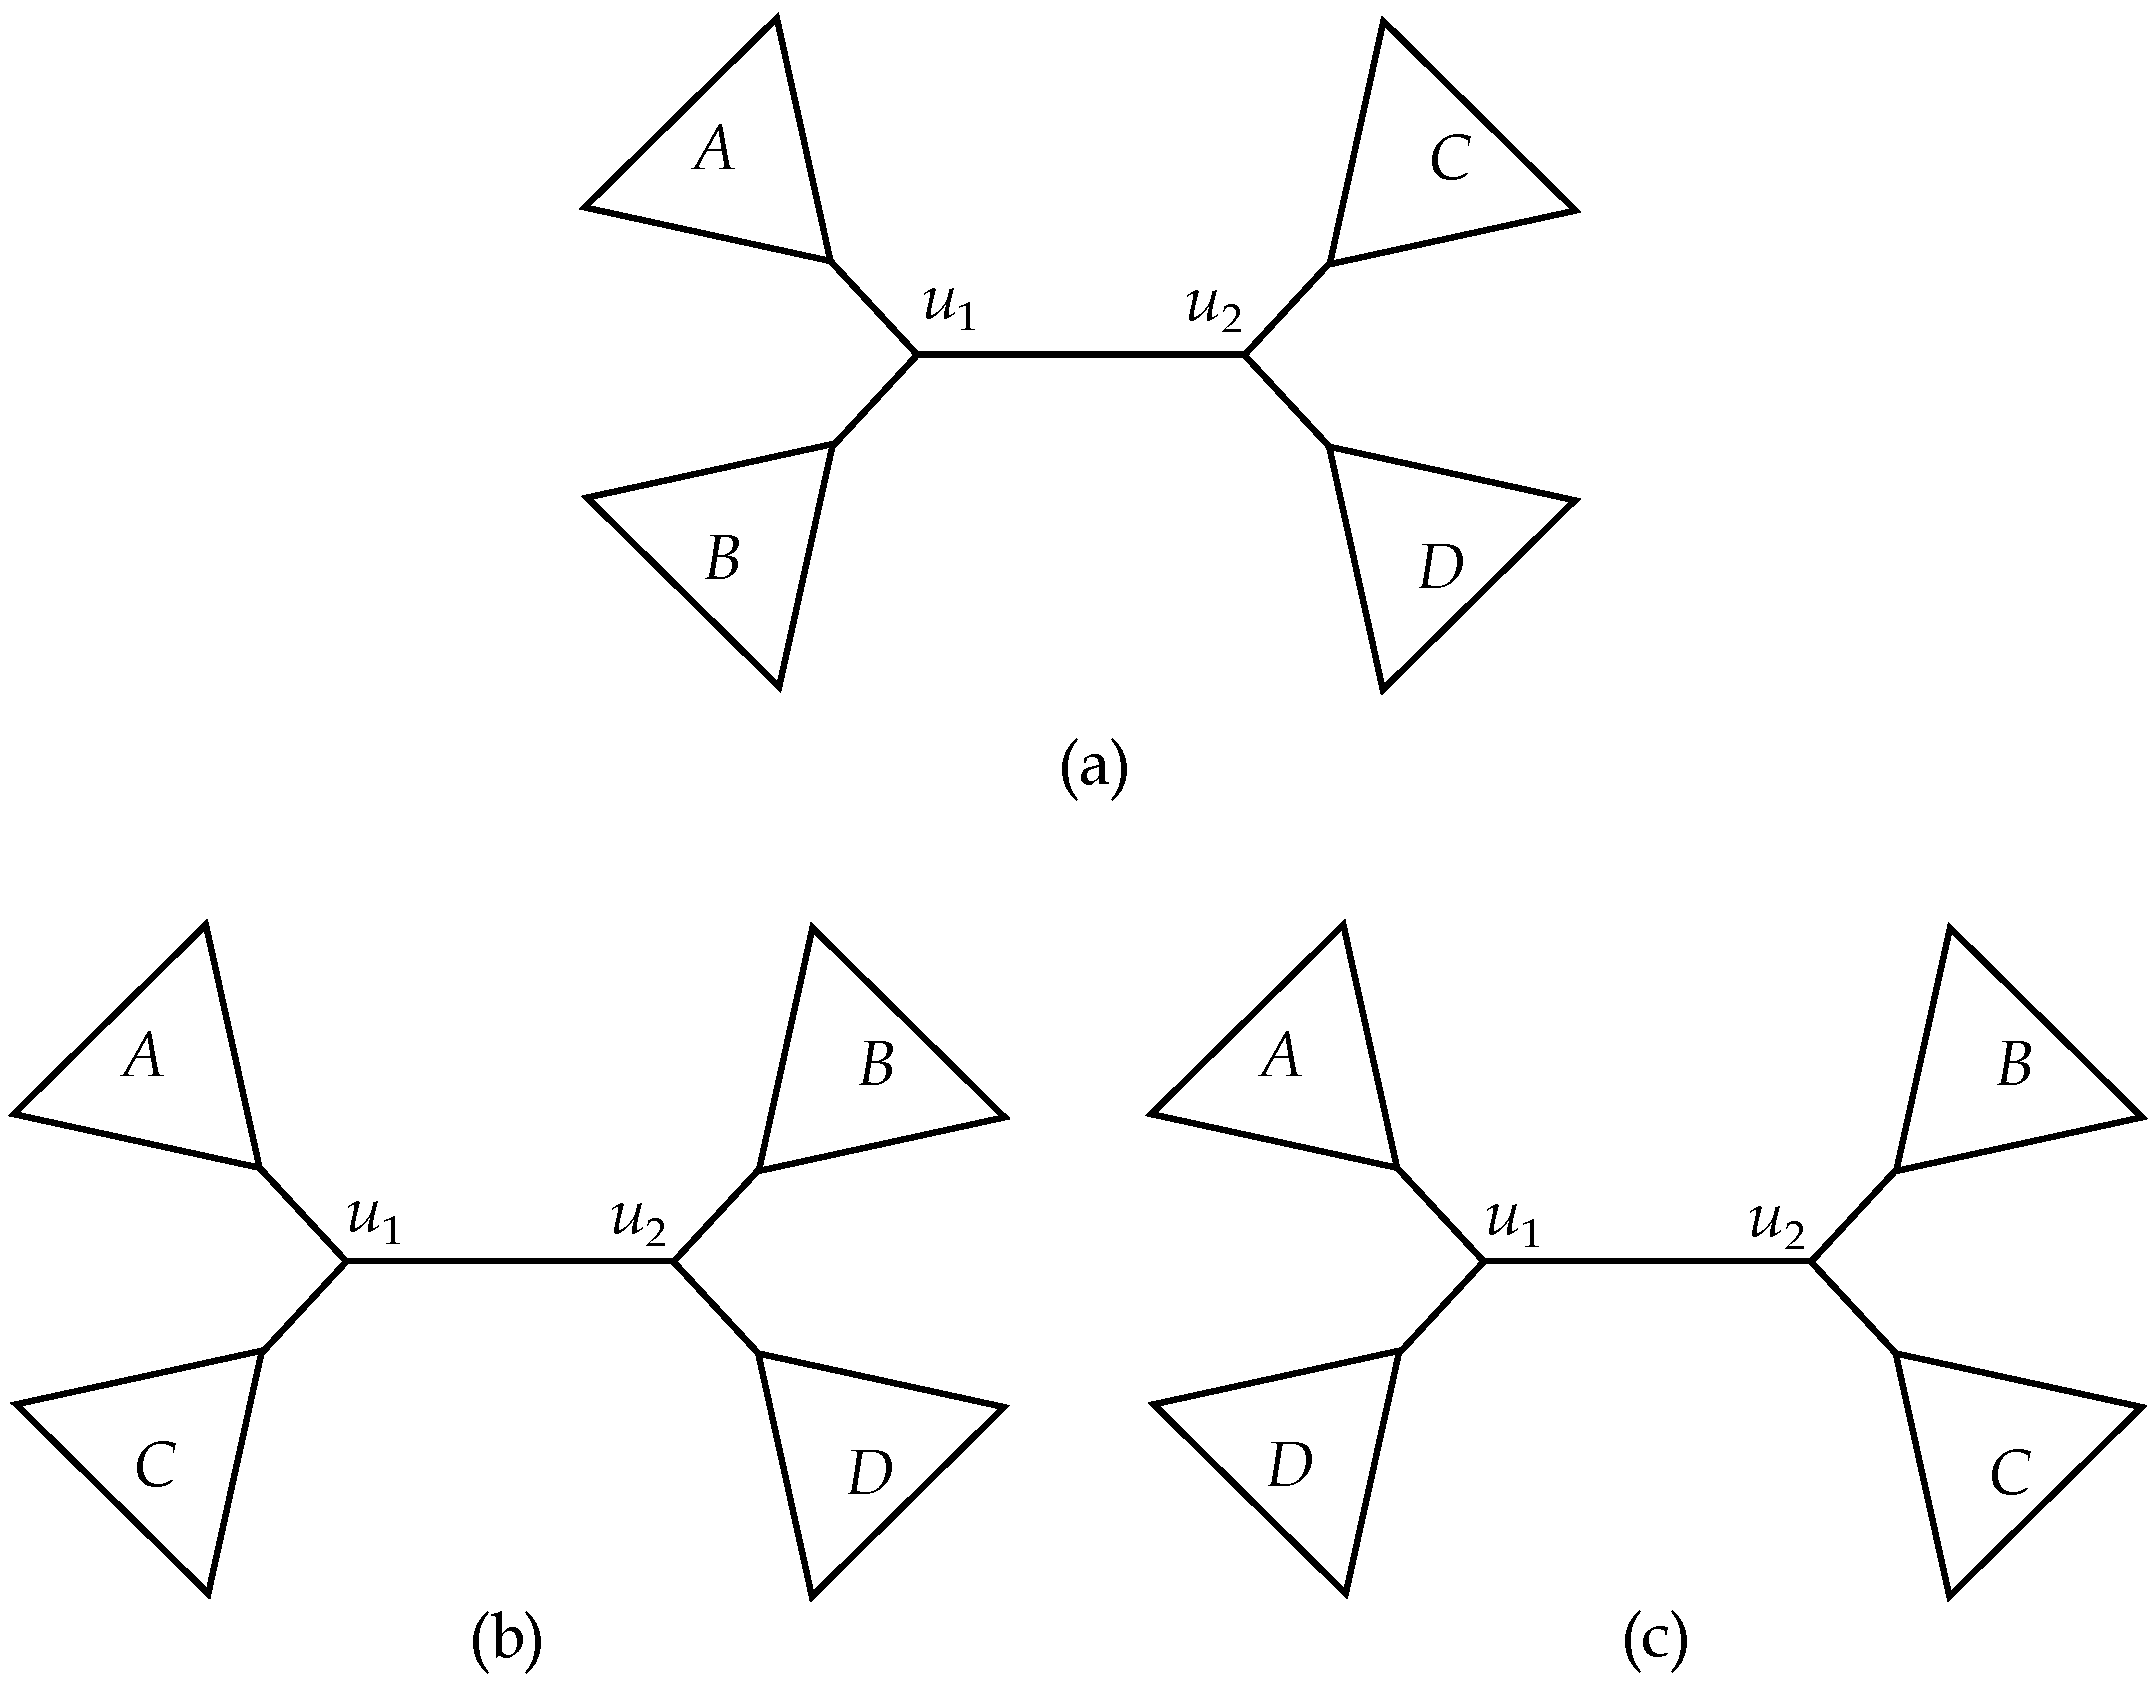
\includegraphics[scale=0.33]{Figure3.pdf}
		\caption{\textbf{Same figure upside down}}
		\label{fg:fg1}
	\end{figure}
\end{document}
